% Copyright (c) 2008-2009 solvethis
% Copyright (c) 2010-2016,2018-2019,2021 Casper Ti. Vector
% Copyright (c) 2021 Kurapica
% Public domain.
%
% 使用前请先仔细阅读 pkuthss 和 biblatex-caspervector 的文档,
% 特别是其中的 FAQ 部分和用红色强调的部分。
% 两者可在终端/命令提示符中用
%   texdoc pkuthss
%   texdoc biblatex-caspervector
% 调出。

% 为使用单页设置,可以在 [] 加入"oneside"选项 
\documentclass[UTF8,oneside]{pkuthss}
% oneside 选项使文档为单面打印,twoside 选项使文档为双面打印。
\usepackage{hyperref}
\hypersetup{colorlinks = true, linkcolor = black, citecolor = black, urlcolor = black}
% 如果的确须要使脚注按页编号的话,可以去掉后面 footmisc 包的注释。
%\usepackage[perpage]{footmisc}

% 使用 biblatex 排版参考文献,并规定其格式(详见 biblatex-caspervector 的文档)。
% 这里按照西文文献在前,中文文献在后排序(“sorting = ecnyt”);
% 若须按照中文文献在前,西文文献在后排序,请设置“sorting = cenyt”;
% 若须按照引用顺序排序,请设置“sorting = none”。
% 若须在排序中实现更复杂的需求,请参考 biblatex-caspervector 的文档。
% biblatex-caspervector 也有一个“ugly”选项,使其更像国标格式;此外也可考虑
% 改用 style = gb7714-2015 并去掉之后两选项,详见 biblatex-gb7714-2015 的文档。
\usepackage[backend = biber, style = caspervector, utf8, sorting = none]{biblatex}


% 在此处添加需要的 packages
\usepackage{multirow}
\usepackage{makecell}
\usepackage{float}
\usepackage{tabularx}
\usepackage{pdfpages}

% 对于 linespread 值的计算过程有兴趣的同学可以参考 pkuthss.cls。
\renewcommand*{\bibfont}{\zihao{5}\linespread{1.27}\selectfont}
% 按学校要求设定参考文献列表的段间距。
\setlength{\bibitemsep}{3bp}

% 如是双盲版论文,将 \blindfalse 改为 \blindtrue。后面可用
% \ifblind 根据是否双盲来条件地启用代码(参见本文件后面部分)。
\newif\ifblind\blindfalse
% 设定文档的基本信息。
\pkuthssinfo{
	cthesisname = {本科生毕业论文}, ethesisname = {Thesis},
	thesiscover = {本科生毕业论文},
	% 长标题可用 \thssnl 强制换行,不能用“\\”(双盲版会出错)。
	ctitle = {测试甲乙丙丁},
	etitle = {Test A B C D},
	% Use ~ to add non-breaking space
	cauthor = {宇航员}, eauthor = {Test}, date = {二〇二五~年~五~月},
	studentid = {2500018888}, school = {信息科学技术学院},
	cmajor = {电子信息工程}, emajor = {Some Major},
	% direction = {某某方向}, % 本科毕业无需填方向
	cmentor = {导师}, ementor = {Prof.\ Somebody},
	ckeywords = {第一,第二,第三},
	ekeywords = {first, second, third},
	% 以下两项无双盲评审需求的用户可保持原状。
	% 注意 discipline/major 分别指一/二级学科。
	% blindid = {9876543210}, discipline = {某某学科}
}
% 载入参考文献数据库(注意不要省略“.bib”)。
\addbibresource{thesis.bib}
\usepackage{listings}
\usepackage{ctex}
\usepackage{tikz}
\usetikzlibrary{arrows.meta, positioning}


% 用来设置附录中代码的样式
\lstset{
    basicstyle          =   \sffamily,          % 基本代码风格
    keywordstyle        =   \bfseries,          % 关键字风格
    commentstyle        =   \rmfamily\itshape,  % 注释的风格,斜体
    stringstyle         =   \ttfamily,  % 字符串风格
    flexiblecolumns,                % 别问为什么,加上这个
    numbers             =   left,   % 行号的位置在左边
    showspaces          =   false,  % 是否显示空格,显示了有点乱,所以不现实了
    numberstyle         =   \zihao{-5}\ttfamily,    % 行号的样式,小五号,tt等宽字体
    showstringspaces    =   false,
    captionpos          =   t,      % 这段代码的名字所呈现的位置,t指的是top上面
    frame               =   lrtb,  
	basicstyle      =   \zihao{-5}\ttfamily,
    numberstyle     =   \zihao{-5}\ttfamily,
    keywordstyle    =   \color{blue},
    keywordstyle    =   [2] \color{teal},
    stringstyle     =   \color{magenta},
    commentstyle    =   \color{red}\ttfamily,
    breaklines      =   true,
    breakatwhitespace = true % 尽量在空格处换行(可选)  % 自动换行,建议不要写太长的行
    columns         =   fixed,  % 如果不加这一句,字间距就不固定,很丑,必须加
    basewidth       =   0.5em, % 显示边框
}

\lstdefinestyle{Python}{
    language        =   Python, % 语言选Python
    basicstyle      =   \zihao{-5}\ttfamily,
    numberstyle     =   \zihao{-5}\ttfamily,
    keywordstyle    =   \color{blue},
    keywordstyle    =   [2] \color{teal},
    stringstyle     =   \color{magenta},
    commentstyle    =   \color{red}\ttfamily,
    breaklines      =   true,
    breakatwhitespace = true % 尽量在空格处换行(可选)  % 自动换行,建议不要写太长的行
    columns         =   fixed,  % 如果不加这一句,字间距就不固定,很丑,必须加
    basewidth       =   0.5em,
}


% 普通用户可删除此段,并相应地删除 chap/*.tex 中的
% “\pkuthssffaq % 中文测试文字。”一行。
\usepackage{color}
\def\pkuthssffaq{%
	\emph{\textcolor{red}{pkuthss 文档模版最常见问题:}}

	\texttt{\string\cite}、\texttt{\string\parencite} %
	和 \texttt{\string\supercite} 三个命令分别产生%
	未格式化的、带方括号的和上标且带方括号的引用标记。
	
	若要避免章末空白页,请在调用 pkuthss 文档类时加入 \texttt{openany} 选项。

	如果编译时不出参考文献,
	请参考 \texttt{texdoc pkuthss}“问题及其解决”一章
	“上游宏包可能引起的问题”一节中关于 biber 的说明。

	因无法假定用户使用哪种方式排版表格,用户须自行保证表格字号符合学校规定。%
}

\begin{document}
	% 以下为正文之前的部分,默认不进行章节编号。
	\frontmatter
	% 此后到下一 \pagestyle 命令之前不排版页眉或页脚。
	\pagestyle{empty}
	% 自动生成封面。
	\ifblind\makeblind\else\maketitle\fi

	% 论文导师评阅表
	% \include{chap/sheet}
	\cleardoublepage
	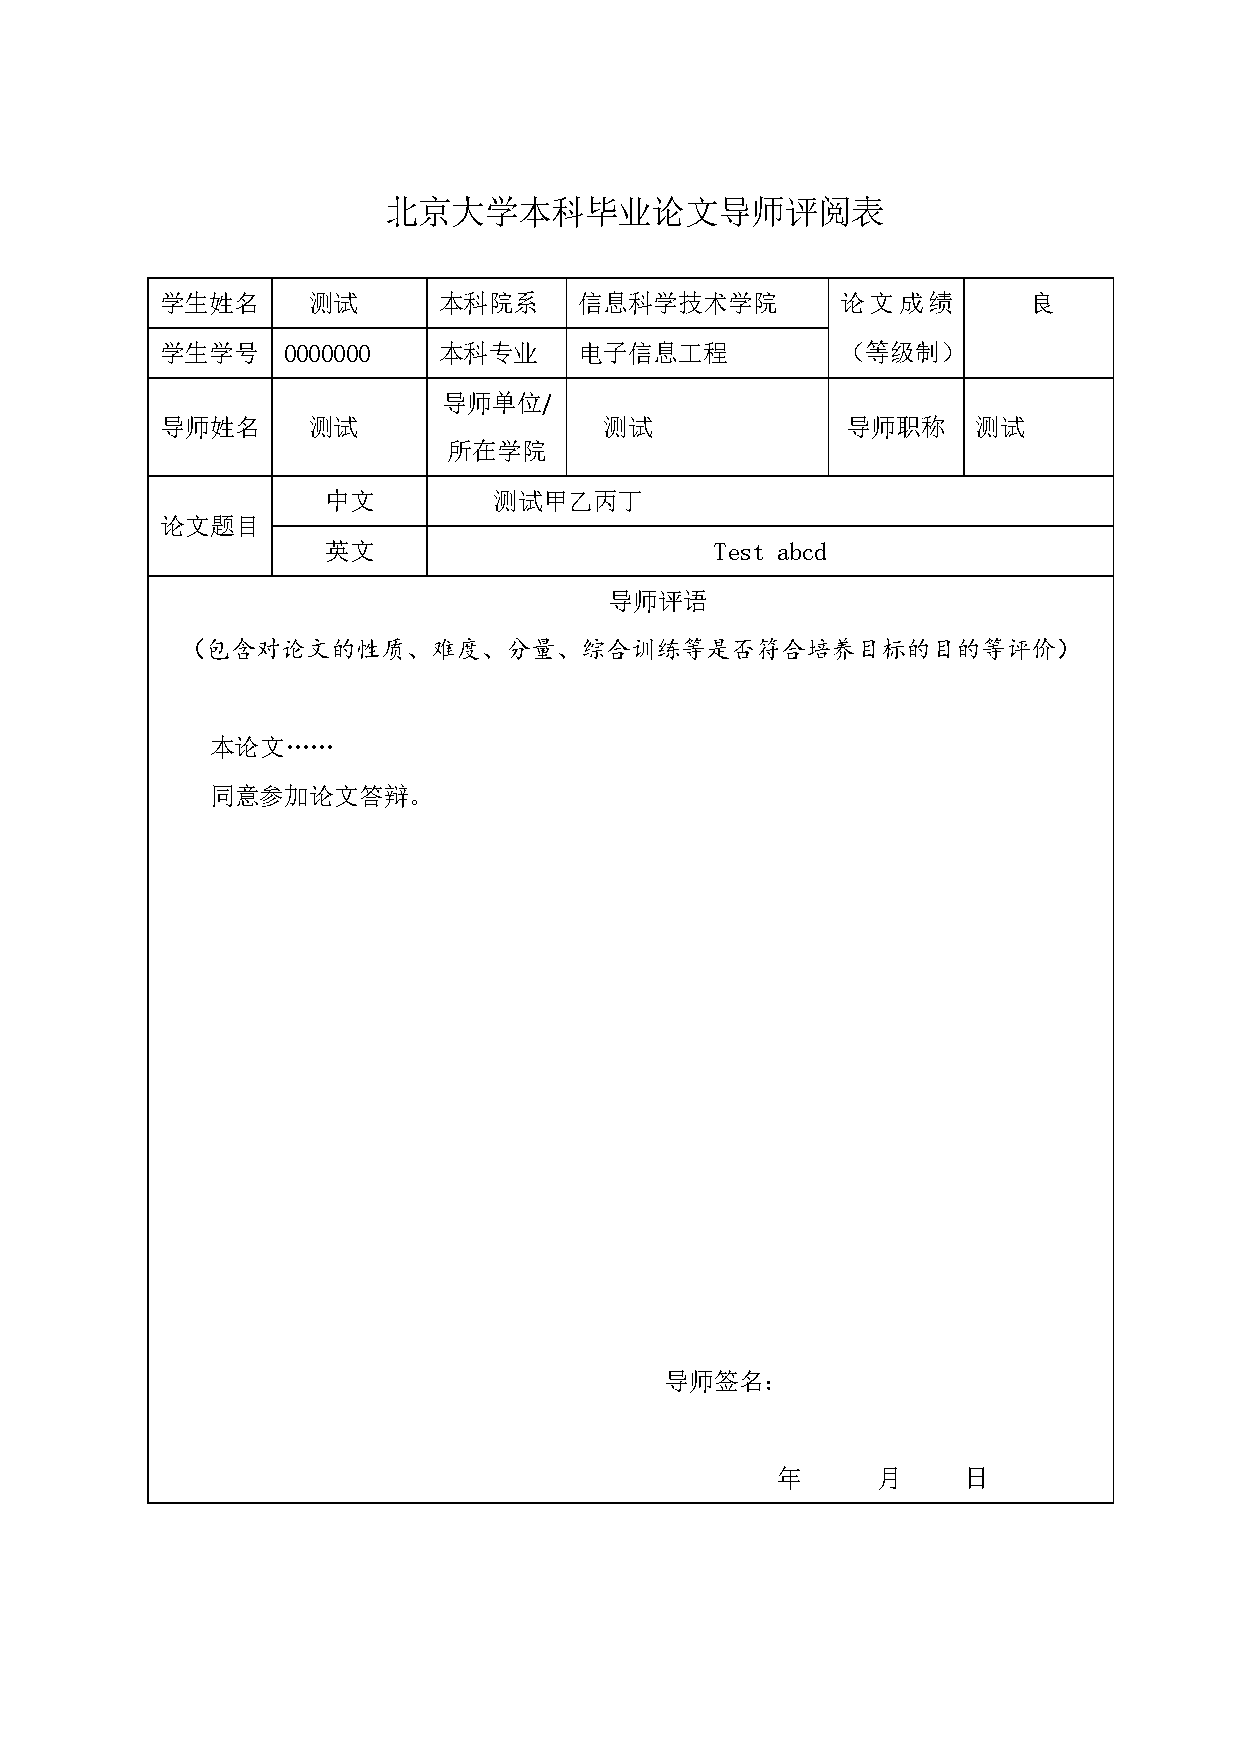
\includepdf[pages=-]{others/sheet.pdf}


	% 版权声明。封面要求单面打印,故须新开右页。
	\cleardoublepage
	% Copyright (c) 2008-2009 solvethis
% Copyright (c) 2010-2017 Casper Ti. Vector
% All rights reserved.
%
% Redistribution and use in source and binary forms, with or without
% modification, are permitted provided that the following conditions are
% met:
%
% * Redistributions of source code must retain the above copyright notice,
%   this list of conditions and the following disclaimer.
% * Redistributions in binary form must reproduce the above copyright
%   notice, this list of conditions and the following disclaimer in the
%   documentation and/or other materials provided with the distribution.
% * Neither the name of Peking University nor the names of its contributors
%   may be used to endorse or promote products derived from this software
%   without specific prior written permission.
%
% THIS SOFTWARE IS PROVIDED BY THE COPYRIGHT HOLDERS AND CONTRIBUTORS "AS
% IS" AND ANY EXPRESS OR IMPLIED WARRANTIES, INCLUDING, BUT NOT LIMITED TO,
% THE IMPLIED WARRANTIES OF MERCHANTABILITY AND FITNESS FOR A PARTICULAR
% PURPOSE ARE DISCLAIMED. IN NO EVENT SHALL THE COPYRIGHT HOLDER OR
% CONTRIBUTORS BE LIABLE FOR ANY DIRECT, INDIRECT, INCIDENTAL, SPECIAL,
% EXEMPLARY, OR CONSEQUENTIAL DAMAGES (INCLUDING, BUT NOT LIMITED TO,
% PROCUREMENT OF SUBSTITUTE GOODS OR SERVICES; LOSS OF USE, DATA, OR
% PROFITS; OR BUSINESS INTERRUPTION) HOWEVER CAUSED AND ON ANY THEORY OF
% LIABILITY, WHETHER IN CONTRACT, STRICT LIABILITY, OR TORT (INCLUDING
% NEGLIGENCE OR OTHERWISE) ARISING IN ANY WAY OUT OF THE USE OF THIS
% SOFTWARE, EVEN IF ADVISED OF THE POSSIBILITY OF SUCH DAMAGE.

% 此处不用 \specialchap,因为学校要求目录不包括其自己及其之前的内容。
\chapter*{版权声明}
% 综合学校的书面要求及 Word 模版来看,版权声明页不用加页眉、页脚。
\thispagestyle{empty}

任何收存和保管本论文各种版本的单位和个人,
未经本论文作者同意,不得将本论文转借他人,
亦不得随意复制、抄录、拍照或以任何方式传播。
否则一旦引起有碍作者著作权之问题,将可能承担法律责任。

% 若须排版二维码,请将二维码图片重命名为“barcode”,
% 转为合适的图片格式,并放在当前目录下,然后去掉下面 2 行的注释。
%\vfill\noindent
%\includegraphics[height = 5em]{barcode}

% vim:ts=4:sw=4


	% 此后到下一 \pagestyle 命令之前正常排版页眉和页脚。
	\cleardoublepage
	\pagestyle{plain}
	% 重置页码计数器,用大写罗马数字排版此部分页码。
	\setcounter{page}{0}
	\pagenumbering{Roman}
	% 中西文摘要。
	% Copyright (c) 2014,2016,2021 Casper Ti. Vector
% Public domain.

\begin{cabstract}
	这是摘要
\end{cabstract}

\ifblind\begin{beabstract}\else\begin{eabstract}\fi
	This is the abstract.
\ifblind\end{beabstract}\else\end{eabstract}\fi

% vim:ts=4:sw=4

	% 自动生成目录。
	\tableofcontents

	% 以下为正文部分,默认要进行章节编号。
	\mainmatter
	% 各章节。
	% Copyright (c) 2014,2016,2018 Casper Ti. Vector
% Public domain.

\chapter{引言}

\section{研究背景}
这里写点研究背景吧。如图\ref{fig:timeline}是latex画框图的示例,
可以用AI辅助生成,或者用visio/ppt等工具画出来再插入图片。

\begin{figure}[htbp]
    \centering
    \begin{tikzpicture}[
        timeline/.style={draw, thick},
        stage/.style={rectangle, draw=blue!50, fill=blue!10, thick, text width=6.5cm, minimum height=2.3cm, align=left, rounded corners},
        year/.style={font=\bfseries},
        node distance=1.2cm
    ]
    
    % 时间轴竖线
    \draw[timeline, -{Latex[length=3mm]}] (0,0) -- (0,-12);
    
    % 时间点及标记
    \foreach \y/\year in {0/1960s末, -4/2000, -8/2025, -12/今}
        \draw[thick] (-0.2,\y) -- (0.2,\y) node[left=10pt, year] {\year};
    
    % 阶段一
    \node[stage, anchor=west] at (2,-1.8) {
      \textbf{阶段一:1} \\
      \textbf{时间:} 1960s末—2000年 \\
      \textbf{代表项目:} 旧的 \\
      \textbf{特点:} 测试
    };
    
    % 阶段二
    \node[stage, anchor=west] at (2,-5.8) {
      \textbf{阶段二:2} \\
      \textbf{时间:} 2000—2025年 \\
      \textbf{代表项目:} 稍旧的 \\
      \textbf{特点:} 测试
    };
    
    % 阶段三
    \node[stage, anchor=west] at (2,-9.8) {
      \textbf{阶段三:3} \\
      \textbf{时间:} 2025年至今 \\
      \textbf{代表项目:} 新的 \\
      \textbf{特点:} 测试
    };
    
    \end{tikzpicture}
    \caption{项目背景发展阶段时间轴图}
    \label{fig:timeline}
\end{figure}

\section{研究意义}
\label{sec:research-significance}
随便写写。加一个引用吧。\supercite{test-zh}。
	% Copyright (c) 2014,2016 Casper Ti. Vector
% Public domain.

\chapter{项目架构}

\section{测试}
\subssection{测试1}
在这里放一个图片。
\begin{figure}[htbp]
    \centering
    
\includegraphics[width=0.5\textwidth]{pic/pkulogo.pdf}
    \caption{测试图片}
    \label{fig:1}
\end{figure}
\subsection{测试2}
这里放一个表格。
\begin{table}[htbp]
    \centering
    \caption{测试表格}
    \begin{tabular}{|c|c|c|}
        \hline
        \textbf{测试1} & \textbf{测试2} & \textbf{测试3} \\
        \hline
        1 & 2 & 3 \\
        4 & 5 & 6 \\
        7 & 8 & 9 \\
        \hline
    \end{tabular}
    \label{tab:1}
\end{table}
	\chapter{具体实现}

\section{测试}
\begin{itemize}
    \item 测试1
    \item 测试2
    \item 测试3
\end{itemize}

\begin{enumerate}
    \item 测试1
    \item 测试2
    \item 测试3
\end{enumerate}

\begin{description}
    \item[测试1] 测试1
    \item[测试2] 测试2
    \item[测试3] 测试3
\end{description}

\section{测试代码}

\begin{lstlisting}[language=python]
def test():
    print("Hello, World!")
test()
\end{lstlisting}
	\chapter{总结与展望}
\section{总结}
\label{sec:summary}
这里写点总结吧。
\section{展望}
\label{sec:prospect}
这里写点展望吧。

	% \include{chap/chap5}
	
	% 正文中的附录部分。
	\appendix
	% 排版参考文献列表。bibintoc 选项使“参考文献”出现在目录中;
	% 如果同时要使参考文献列表参与章节编号,可将“bibintoc”改为“bibnumbered”。
	\printbibliography[heading = bibintoc]
	% 各附录。
	% Copyright (c) 2014,2016 Casper Ti. Vector
% Public domain.

\chapter{}

\section*{附录A.1 \quad 测试}
% \pkuthssffaq 
\begin{table}[H]
        \centering
        \caption{测试表格}
        \begin{tabular}{|c|c|c|}
                \hline
                \textbf{测试1} & \textbf{测试2} & \textbf{测试3} \\
                \hline
                1 & 2 & 3 \\
                4 & 5 & 6 \\
                7 & 8 & 9 \\
                \hline
        \end{tabular}
        \label{tab:2}
\end{table}
\section*{附录A.2 \quad 测试}
\pkuthssffaq

	% 以下为正文之后的部分,默认不进行章节编号。
	\backmatter
	
	% 致谢。
	\ifblind\else% Copyright (c) 2014,2016 Casper Ti. Vector
% Public domain.

\chapter{致谢}
谢谢大家!

% vim:ts=4:sw=4
\fi
	% 原创性声明和使用授权说明。
	% % Copyright (c) 2008-2009 solvethis
% Copyright (c) 2010-2017,2021 Casper Ti. Vector
% Copyright (c) 2021 Kurapica
% All rights reserved.
%
% Redistribution and use in source and binary forms, with or without
% modification, are permitted provided that the following conditions are
% met:
%
% * Redistributions of source code must retain the above copyright notice,
%   this list of conditions and the following disclaimer.
% * Redistributions in binary form must reproduce the above copyright
%   notice, this list of conditions and the following disclaimer in the
%   documentation and/or other materials provided with the distribution.
% * Neither the name of Peking University nor the names of its contributors
%   may be used to endorse or promote products derived from this software
%   without specific prior written permission.
%
% THIS SOFTWARE IS PROVIDED BY THE COPYRIGHT HOLDERS AND CONTRIBUTORS "AS
% IS" AND ANY EXPRESS OR IMPLIED WARRANTIES, INCLUDING, BUT NOT LIMITED TO,
% THE IMPLIED WARRANTIES OF MERCHANTABILITY AND FITNESS FOR A PARTICULAR
% PURPOSE ARE DISCLAIMED. IN NO EVENT SHALL THE COPYRIGHT HOLDER OR
% CONTRIBUTORS BE LIABLE FOR ANY DIRECT, INDIRECT, INCIDENTAL, SPECIAL,
% EXEMPLARY, OR CONSEQUENTIAL DAMAGES (INCLUDING, BUT NOT LIMITED TO,
% PROCUREMENT OF SUBSTITUTE GOODS OR SERVICES; LOSS OF USE, DATA, OR
% PROFITS; OR BUSINESS INTERRUPTION) HOWEVER CAUSED AND ON ANY THEORY OF
% LIABILITY, WHETHER IN CONTRACT, STRICT LIABILITY, OR TORT (INCLUDING
% NEGLIGENCE OR OTHERWISE) ARISING IN ANY WAY OUT OF THE USE OF THIS
% SOFTWARE, EVEN IF ADVISED OF THE POSSIBILITY OF SUCH DAMAGE.

{
	\ctexset{section = {
		format+ = {\centering}, beforeskip = {40bp}, afterskip = {15bp}
	}}
	\specialchap{北京大学学位论文原创性声明和使用授权说明}

	% 学校书面要求本页面不要页码,但在给出的 Word 模版中又有页码。
	% 此处以学校书面要求为准。
	\thispagestyle{empty}
	\mbox{}\vspace*{-3em}
	\section*{原创性声明}

	本人郑重声明:
	所呈交的学位论文,是本人在导师的指导下,独立进行研究工作所取得的成果。
	除文中已经注明引用的内容外,
	本论文不含任何其他个人或集体已经发表或撰写过的作品或成果。
	对本文的研究做出重要贡献的个人和集体,均已在文中以明确方式标明。
	本声明的法律结果由本人承担。
	\vskip 1em
	\rightline{%
		论文作者签名:\hspace{5em}%
		日期:\hspace{2em}年\hspace{2em}月\hspace{2em}日%
	}

	\section*{%
		学位论文使用授权说明\\[-0.33em]
		\textmd{\zihao{5}(必须装订在提交学校图书馆的印刷本)}%
	}

	本人完全了解北京大学关于收集、保存、使用学位论文的规定,即:
	\begin{itemize}
		\item 按照学校要求提交学位论文的印刷本和电子版本;
		\item 学校有权保存学位论文的印刷本和电子版,
			并提供目录检索与阅览服务,在校园网上提供服务;
		\item 学校可以采用影印、缩印、数字化或其它复制手段保存论文;
		\item 因某种特殊原因须要延迟发布学位论文电子版,
			授权学校在 $\Box$\nobreakspace{}一年 /
			$\Box$\nobreakspace{}两年 /
			$\Box$\nobreakspace{}三年以后在校园网上全文发布。
	\end{itemize}
	\centerline{(保密论文在解密后遵守此规定)}
	\vskip 1em
	\rightline{%
		论文作者签名:\hspace{5em}导师签名:\hspace{5em}%
		日期:\hspace{2em}年\hspace{2em}月\hspace{2em}日%
	}

	% 若须排版二维码,请将二维码图片重命名为“barcode”,
	% 转为合适的图片格式,并放在当前目录下,然后去掉下面 2 行的注释。
	%\vfill\noindent
	%\includegraphics[height = 5em]{barcode}
}

% vim:ts=4:sw=4

	
\includepdf[pages=-]{others/end.pdf}
\end{document}

% vim:ts=4:sw=4
